\PassOptionsToPackage{table}{xcolor}
\documentclass[t]{beamer}

\usepackage[T1]{fontenc}
\usepackage[utf8]{inputenc}
\usepackage[brazil]{babel}
%\usepackage[round,authoryear]{natbib}
\usepackage[square,sort,numbers]{natbib}
\usepackage{tabulary}
\usepackage[table]{xcolor}
\usepackage{gensymb}
\usepackage{multicol}
\usepackage{multirow}

%%%% TEMAS %%%%
%\usetheme{Antibes}
%\usetheme{Bergen}
%\usetheme{Berkeley}
%\usetheme{Berlin}
%\usetheme{Copenhagen}
%\usetheme{Darmstadt}
%\usetheme{Dresden}
%\usetheme{Frankfurt}
%\usetheme{Goettingen}
%\usetheme{Hannover}
%\usetheme{Ilmenau}
%\usetheme{JuanLesPins}
%\usetheme{Luebeck}
%\usetheme{Madrid}
%\usetheme{Malmoe}
%\usetheme{Marburg}
%\usetheme{Montpellier}
%\usetheme{PaloAlto}
%\usetheme{Pittsburgh}
%\usetheme{Rochester}
\usetheme{Singapore}
%\usetheme{Szeged}
%\usetheme{Warsaw}
%\usetheme{boxes}
%\usetheme{default}
%\usetheme{CambridgeUS}

%%%% CORES %%%%

%\usecolortheme{default}
%\usecolortheme{albatross}
%\usecolortheme{beaver}
%\usecolortheme{beetle}
%\usecolortheme{crane}
%\usecolortheme{dolphin}

\usecolortheme{dove}

%\usecolortheme{fly}
%\usecolortheme{lily}
%\usecolortheme{orchid}
%\usecolortheme{rose}

%\usecolortheme{seagull}

%\usecolortheme{seahorse}

%\usecolortheme{whale}
%\usecolortheme{wolverine}

\setbeamertemplate{navigation symbols}{}%remove navigation symbols

\addtobeamertemplate{navigation symbols}{}{%
    \usebeamerfont{footline}%
    \usebeamercolor[fg]{footline}%
    \hspace{1em}%
    \insertframenumber/\inserttotalframenumber
}

%%%% TITULO %%%%
\institute[Universities Here and There] % (optional)
{
  Programa de Pós-graduação em Informática\\
  Instituto de Computação\\
  Universidade Federal do Amazonas
}
\title % (optional, only for long titles)
{Detecção de elementos antrópicos em imagens aéreas da floresta amazônica}
%\subtitle{Evidence from India}
\author %[Author, Anders] % (optional, for multiple authors)
{Luiz Carlos A. M. Cavalcanti
\\Orientadora: Dr$^a$ Eulanda Miranda dos Santos} %\inst{1}}
\date[] % (optional)
{}
\subject{Computer Science}

\AtBeginSection[]
{
  \begin{frame}
    \frametitle{Roteiro}
    \tableofcontents[currentsection]
  \end{frame}
}

\begin{document}
  \begin{frame}\titlepage\end{frame}

%%%%%%%%%%%%%%%

\section{Contextualização}

\begin{frame}[c]
\frametitle{Introdução}

	\begin{minipage}{0.7\linewidth}
		Amazônia legal:
		\begin{itemize}
			\item 11 mil km de fronteiras;
			\item 22 mil km de vias fluviais;
			\item 66\% do território nacional.
		\end{itemize}

		\vspace{0.5cm}

		VANTs podem ser usados no patrulhamento:
		\begin{itemize}
			\item Diminuição do risco humano;
			\item Maior cobertura de área;
			\item Aproximação discreta;
			\item Variedade de sensores embarcados.
		\end{itemize}
	\end{minipage}
	\begin{minipage}{0.28\linewidth}
		\begin{figure}[h]
			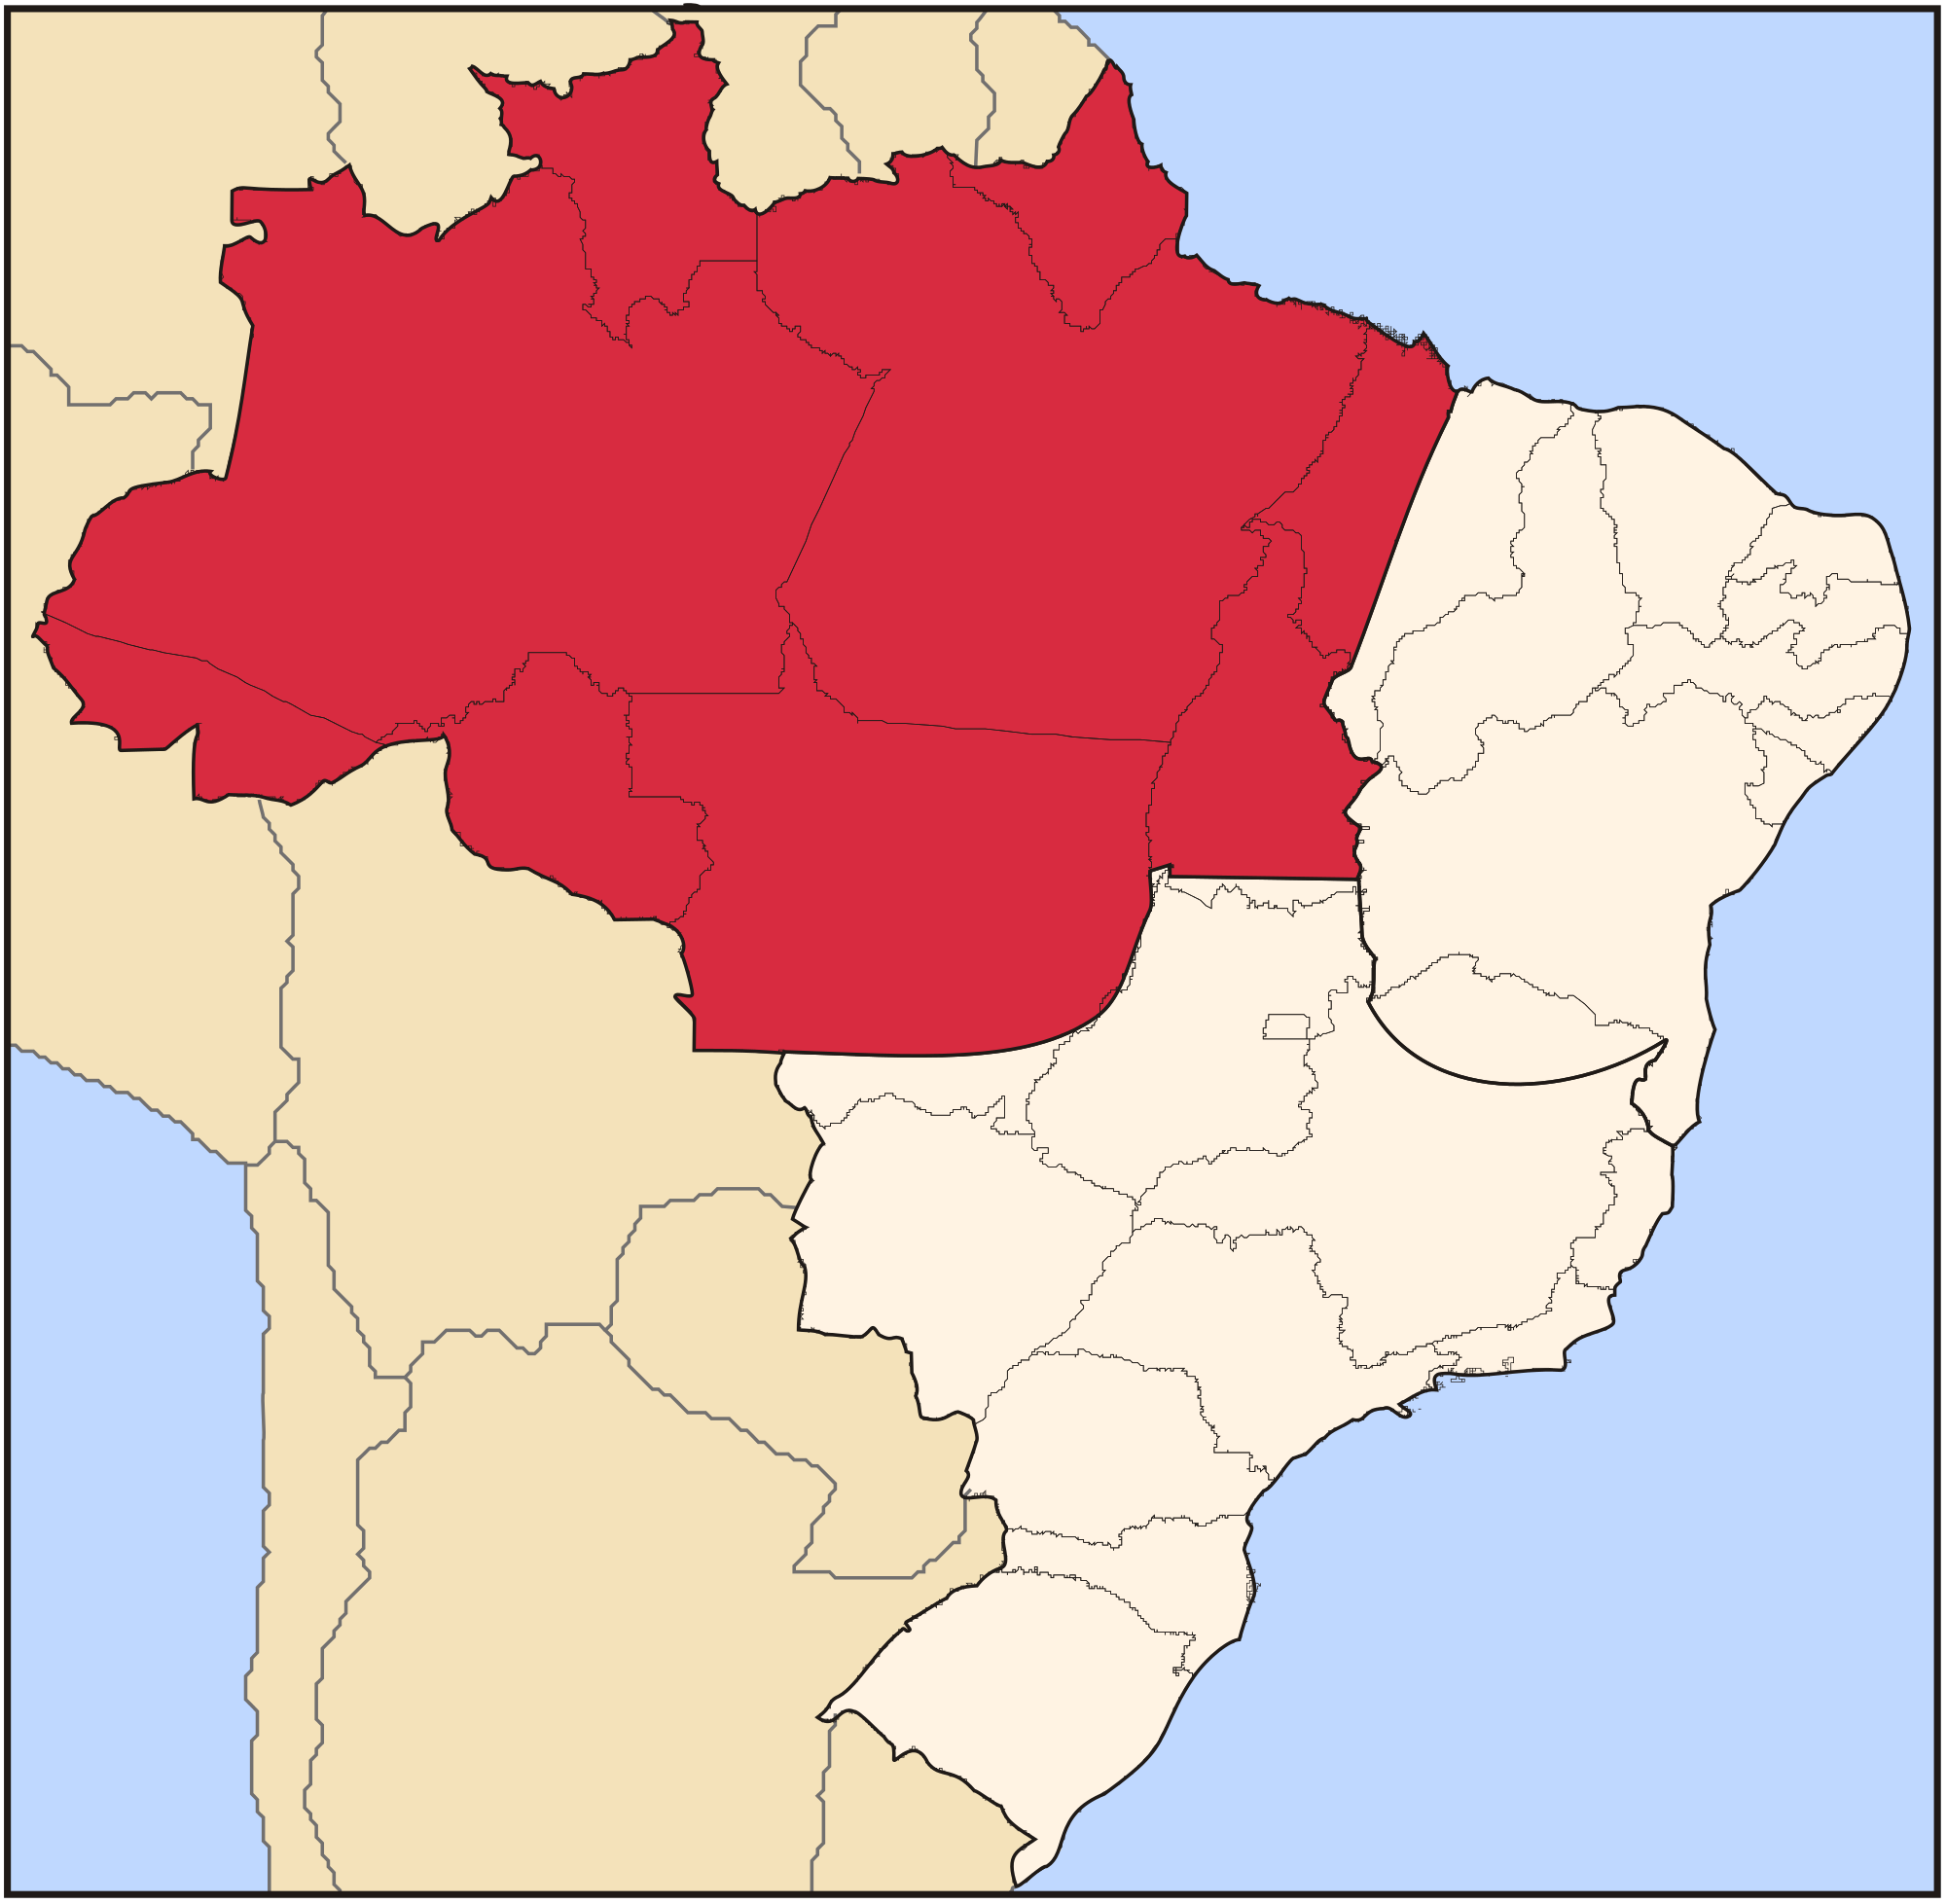
\includegraphics[width=\textwidth]{imgs/amazonia_legal}
		\end{figure}

		\begin{figure}[h]
			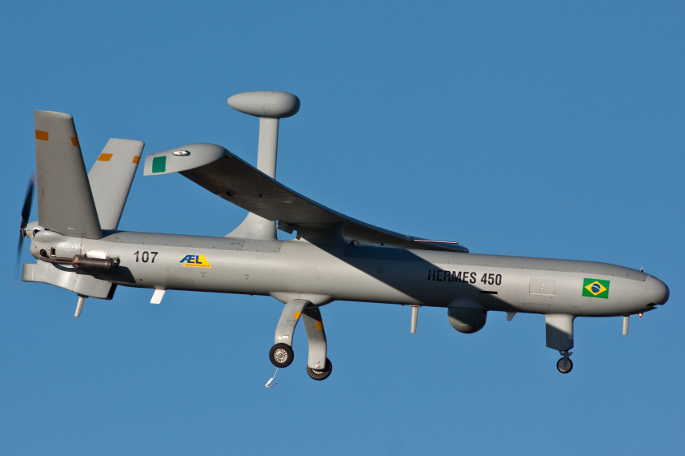
\includegraphics[width=\textwidth]{imgs/hermes}
		\end{figure}
	\end{minipage}
\end{frame}

\begin{frame}[c]
\frametitle{Motivação}

A nova quantidade de dados causa problemas. É desejável uma solução computacional que proporcione:

\begin{itemize}
	\item Maior rapidez na análise de dados;
	\item Redução da quantidade de informação a analizar;
	\item Necessidade de menos especialistas por missão.
\end{itemize}

Objetos de interesse:
	\begin{figure}[h]
		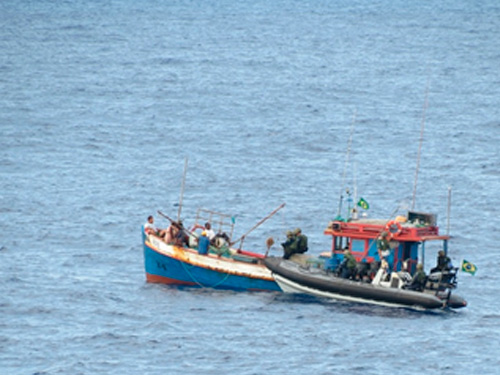
\includegraphics[width=.3\textwidth]{imgs/pesca_ilegal}
		\hspace{0.1cm}
		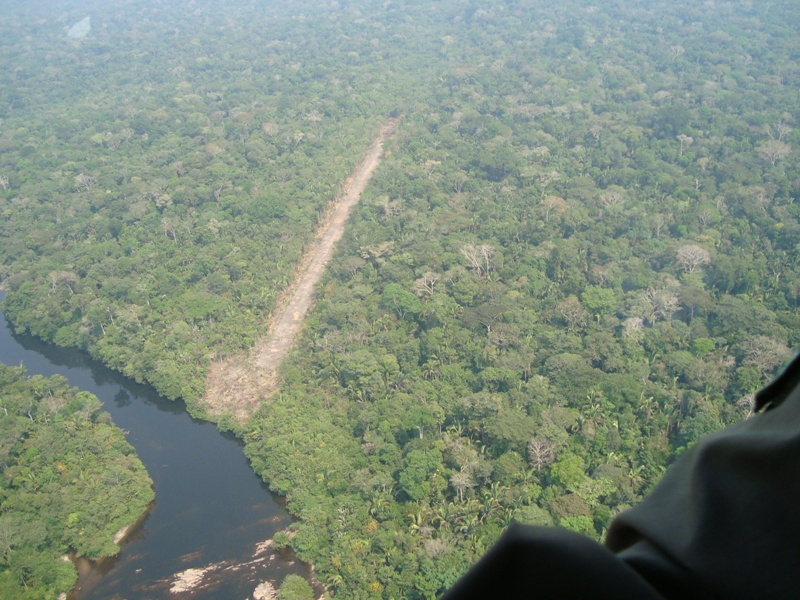
\includegraphics[width=.3\textwidth]{imgs/pista_de_pouso}
		\hspace{0.1cm}
		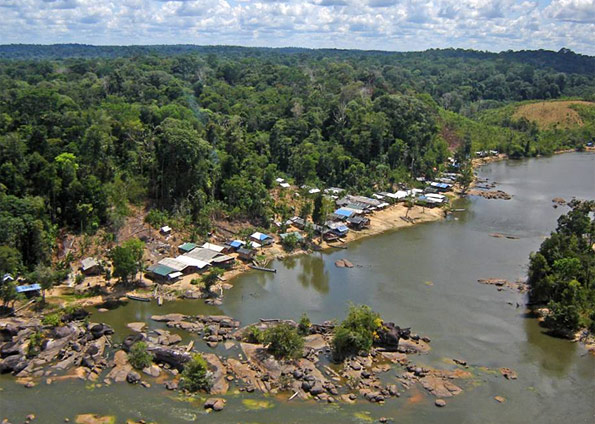
\includegraphics[width=.32\textwidth]{imgs/garimpo}
	\end{figure}

\end{frame}

\begin{frame}[c]
\frametitle{Objetivo geral}
	Propor e validar uma abordagem utilizando processamento digital de imagens e aprendizagem de máquina para detecção automática de elementos antrópicos em imagens aéreas da floresta amazônica.
\end{frame}

\begin{frame}[c]
\frametitle{Objetivos específicos}

\begin{itemize}
    \item Organizar uma base de imagens devidamente rotuladas que sirva de referência para futuros estudos desta problemática;
    \item Definir métodos para segmentação de imagens aéreas da floresta amazônica;
    \item Definir métodos para extração e seleção de características mais adequadas ao problema em questão.
    \item Apontar o melhor conjunto de técnicas para a detecção de elementos antrópicos em imagens aéreas da floresta amazônica.
\end{itemize}

\end{frame}

%%%%%%%%%%%%%%%

\section{Trabalhos relacionados}

\begin{frame}[c]
	\frametitle{Trabalhos relacionados}

	O levantamento bibliográfico foi feito a partir de três temas de pesquisa:
	\vspace{0.5cm}
	\begin{itemize}
		\item Segmentação de imagens;
		\item Classificação de imagens aéreas;
		\item Detecção de anomalias em imagens.
	\end{itemize}
\end{frame}

\begin{frame}[c]
	\frametitle{Trabalhos relacionados: Segmentação de imagens}

	\textbf{\textit{Berkeley Segmentation Dataset 500} (BSD500)}
	
	\begin{figure}[h]
		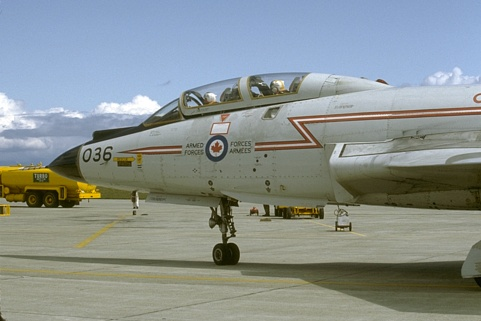
\includegraphics[width=.3\textwidth]{imgs/bsd500_1}
		\hspace{0.1cm}
		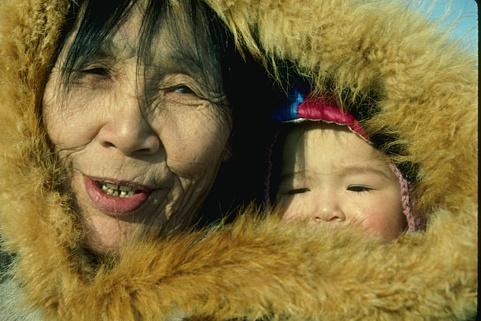
\includegraphics[width=.3\textwidth]{imgs/bsd500_2}
		\hspace{0.1cm}
		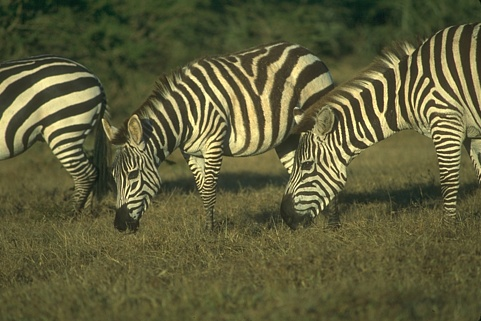
\includegraphics[width=.3\textwidth]{imgs/bsd500_3}
	\end{figure}

	\textit{Arbelaez et al. (2011)}

	\vspace{.5cm}
	
	Conjunto de 500 imagens naturais. Todas as imagens possuem \textit{ground truth} de segmentação por seres humanos.

	\vspace{.5cm}

	Uma importante base de imagens naturais para comparação entre algoritmos de segmentação.

\end{frame}

\begin{frame}[c]
	\frametitle{Trabalhos relacionados: Segmentação de imagens}

	\textbf{Systematic benchmarking of aerial image segmentation}

	\textit{Yuan, Gleason e Cheriyadat (2013)}

	\begin{figure}[h]
		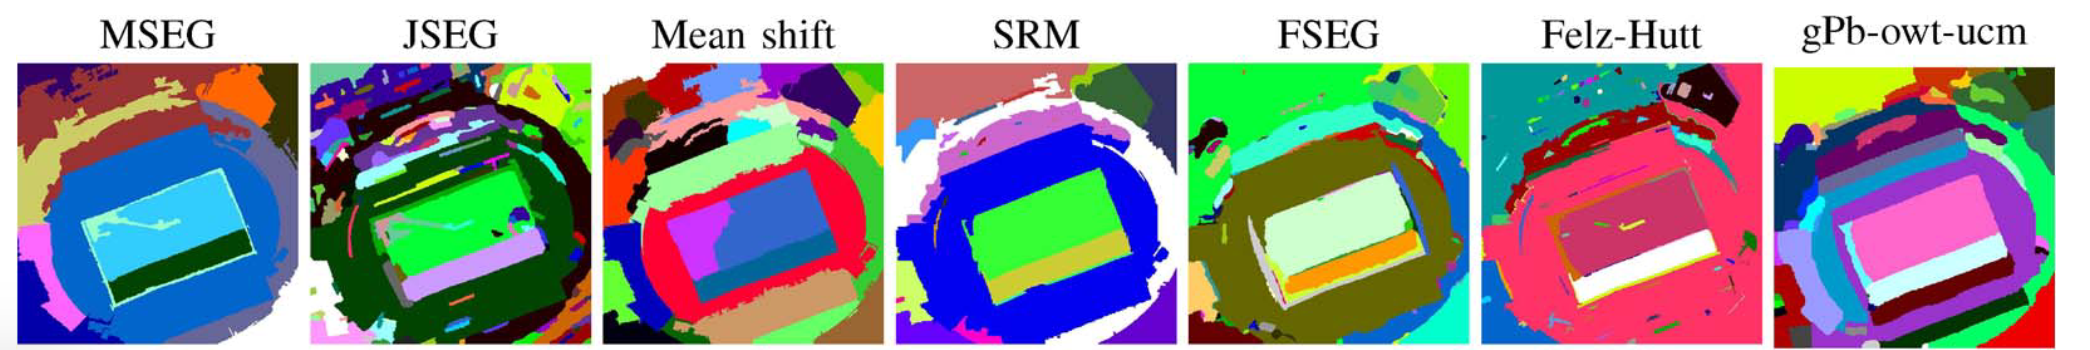
\includegraphics[width=\textwidth]{imgs/yuan_2013}
	\end{figure}

	\small{
	\begin{table}[h]
	\centering
	\begin{tabulary}{\linewidth}{|L|L|C|C|}
	\hline
	\textbf{Técnica} & \textbf{Características} & \textbf{Pr. bordas} & \textbf{Pr. regiões } \\ \hline
%	Manual      & \hspace{1cm} -       & 69\% & 84\% \\ \hline
	gPb-owt-ucm & Brilho, cor, textura & \cellcolor{gray!25} 65\% & \cellcolor{gray!25} 69\% \\ \hline
	FSEG        & Textura              & 61\% & 66\% \\ \hline
	SRM         & Cor, intensidade     & 60\% & 60\% \\ \hline
	JSEG        & Cor, borda           & 56\% & 66\% \\ \hline
	MSEG        & Cor, morfologia      & 57\% & 50\% \\ \hline
	Mean-shift  & Cor, posição         & 58\% & 48\% \\ \hline
	\end{tabulary}
	\end{table}
	}
\end{frame}

%\begin{frame}
%	\frametitle{Trabalhos relacionados: Segmentação de imagens}
%
%	\vspace{0.2cm}
%
%	\textbf{Unsupervised segmentation of color-texture regions in images and video}
%
%	\textit{Deng e Manjunath (2001)}
%	
%	\begin{figure}[h]
%  		\centering
%		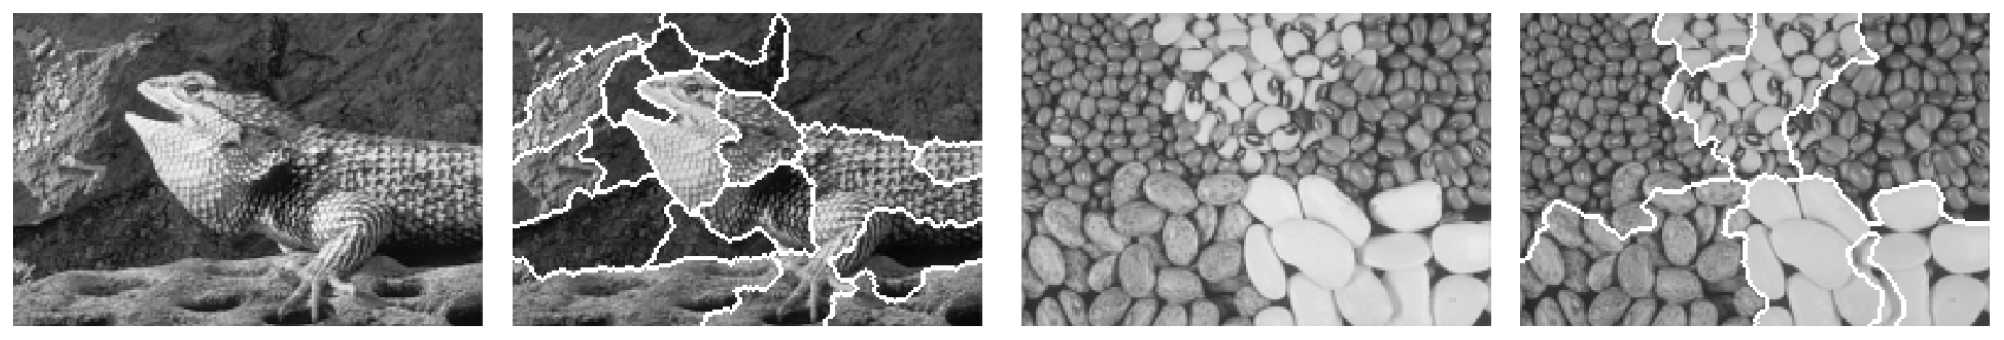
\includegraphics[scale=0.25]{imgs/demo_jseg}
%	\end{figure}
%
%	Descreve o algoritmo JSEG, que segmenta a imagem em duas etapas:
%	\begin{enumerate}
%		\item Quantização das cores em diversas classes;
%		\item Computação de um limiar ($J$) para determinar as bordas a partir das cores quantizadas.
%	\end{enumerate}
%
%	As regiões são obtidas a partir de crescimento de região com base no valor de $J$.
%
%\end{frame}

%\begin{frame}
%	\frametitle{Trabalhos relacionados: Segmentação de imagens}
%
%	\textbf{Mean shift: a robust approach toward feature space analysis}
%
%	\textit{Comaniciu e Meer (2002)}
%
%	\vspace{0.5cm}
%
%	O algoritmo computa vetores de mean-shift iterativamente para mapear pixels para o domínio espacial e de cores do centro de seus \textit{clusters}. Após a convergência, os \textit{clusters} são fundidos de acordo com parâmetros de similaridade. 
%
%	\vspace{0.5cm}
%
%	Parâmetros como largura de banda espacial, de cores e o tamanho do menor \textit{cluster} podem ser utilizados para adequar o algoritmo ao problema em questão.
%
%\end{frame}

%\begin{frame}
%	\frametitle{Trabalhos relacionados: Segmentação de imagens}
%
%	\textbf{Efficient graph-based image segmentation}
%
%	\textit{Felzenszwalb e Huttenlocher (2004)}
%
%	\vspace{0.5cm}
%
%	O algoritmo MSEG é amplamente usado pela comunidade de sensoriamento remoto.
%
%	\vspace{0.5cm}
%
%	Sob a óptica de grafos, os pixels são tratados como nodos e os pesos de suas arestas representam a diferença entre características entre os pixels. Um segmento corresponde a um componente conectado.
%\end{frame}
%
%\begin{frame}
%	\frametitle{Trabalhos relacionados: Segmentação de imagens}
%
%	\textbf{Statistical region merging}
%
%	\textit{Nock e Nielsen (2004)}
%
%	\vspace{0.5cm}
%
%	O algoritmo SRM utiliza um procedimento simples de junção acompanhado por uma operação de ordenação para segmentar imagens com eficiência. Duas regiões são unidas se a diferença entre os valores médios dos pixels das duas regiões estão abaixo de um limiar. 
%
%	\vspace{0.5cm}
%
%	A coesão da segmentação pode ser controlada por um parâmetro definido pelo usuário.
%
%\end{frame}
%
%\begin{frame}
%	\frametitle{Trabalhos relacionados: Segmentação de imagens}
%
%	\textbf{Contour Detection and Hierarchical Image Segmentation}
%
%	\textit{Arbelaez et al. (2011)}
%
%	\vspace{0.5cm}
%
%	O algoritmo gPb-owt-ucm realiza segmentação em várias etapas. Primeiramente a técnica combina informações de intensidade, textura e coloração para computar vetores que servirão como detectores de contorno. Posteriormente, uma técnica de \textit{watershed} é aplicada à saída do detector de contornos para produzir uma segmentação hierárquica da imagem.
%
%\end{frame}
%
%\begin{frame}
%	\frametitle{Trabalhos relacionados: Segmentação de imagens}
%
%	\textbf{Factorization-based texture segmentation}
%
%	\textit{Yuan e Wang (2013)}
%
%	\vspace{0.5cm}
%
%	O FSEG primeiramente computa o histograma espectral para cada pixel da imagem. A proposta é que cada característica pode ser aproximada por uma combinação linear de diversas características representativas e suas combinações ponderadas. 
%
%	\vspace{0.5cm}
%
%	Por fim, um pixel é dito pertencente à região com maior peso. O algoritmo FSEG utiliza decomposição de valores singulares e fatoração de matrizes não-negativas para aumentar a eficiência computacional da segmentação.
%
%\end{frame}
%
%\begin{frame}
%	\frametitle{Trabalhos relacionados: Segmentação de imagens}
%
%	Resultados em \textbf{Yuan, Gleason e Cheriyadat (2013)}:
%
%	\small{
%	\begin{table}[h]
%	\centering
%	\begin{tabulary}{\linewidth}{|L|L|C|C|}
%	\hline
%	\textbf{Técnica} & \textbf{Características} & \textbf{Prec. bordas} & \textbf{Prec. regiões } \\ \hline
%	Manual      & \hspace{1cm} -    & 69\% & 84\% \\ \hline
%	gPb-owt-ucm & Cor, borda       & 65\% & 69\% \\ \hline
%	FSEG        & Textura          & 61\% & 66\% \\ \hline
%	SRM         & Cor, intensidade & 60\% & 60\% \\ \hline
%	JSEG        & Cor, borda       & 56\% & 66\% \\ \hline
%	MSEG        & Cor, morfologia  & 57\% & 50\% \\ \hline
%	Mean-shift  & Cor, posição     & 58\% & 48\% \\ \hline
%	\end{tabulary}
%	\end{table}
%	}
%
%\end{frame}

\begin{frame}[c]
	\frametitle{Trabalhos relacionados: Classificação de imagens aéreas}

	Os trabalhos foram selecionados por estar de acordo com as seguintes características das imagens utilizadas:

	\begin{itemize}
		\item Cenas naturais;
		\item Forte presença de vegetação.
 		\item Ortogonais ao solo ou inclinadas à aproximadamente 90\degree;
	\end{itemize}
\end{frame}

%\begin{frame}
%	\frametitle{Trabalhos relacionados: Classificação de imagens aéreas}
%
%	\textbf{Color and texture fusion: application to aerial image segmentation and GIS updating}
%
%	\textit{Dubuisson-Jolly e Gupta (2000)}
%
%	\vspace{0.5cm}
%
%	Apresenta uma técnica de segmentação focada em imagens aéreas coloridas que realiza a segmentações separadamente por cor e textura, para no final unir as duas e chegar a uma segmentação final utilizando um algoritmo de classificação por \textit{Maximum Likelihood}.
%
%\end{frame}
%
%\begin{frame}
%	\frametitle{Trabalhos relacionados: Classificação de imagens aéreas}
%
%	\textbf{Aerial image processing and object recognition}
%
%	\textit{Sadgal, Fazziki e Ouahman (2005)}
%
%	\vspace{0.5cm}
%
%	Sugere pré-processamento, segmentação e reconhecimento em uma única etapa. Combina métodos estocásticos (inferência Bayesiana, campos de Markov) e não-estocásticos (redes neurais).
%
%	\vspace{0.5cm}
%
%	Métodos são unidos no final do processo, permitindo parelelização de boa parte da solução.
%
%\end{frame}
%
%\begin{frame}
%	\frametitle{Trabalhos relacionados: Classificação de imagens aéreas}
%
%	\textbf{A simple and efficient method for segmentation and classification of aerial images}
%
%	\textit{Ahmadi (2013)}
%
%	\vspace{0.5cm}
%
%	Utiliza características de cor (HSV) e textura (filtro de Gabor) e KNN para  realizar classificação de tipos de terreno em imagens aéreas.
%
%\end{frame}
%
%\begin{frame}
%	\frametitle{Trabalhos relacionados: Classificação de imagens aéreas}
%
%	\textbf{Fast semantic segmentation of aerial images based on color and texture}
%
%	\textit{Ghiasi e Amirfattahi (2013)}
%
%	\vspace{0.5cm}
%
%	Realiza segmentação e classificação de tipos de terreno em imagens aéreas.
%
%	\vspace{0.5cm}
%
%	A imagem é dividida em superpixels (fluxos geométricos de Levishtein) e características de cor (RGB) e textura (LBP-HF) são extraídas. Cada superpixel é classificado com KNN.
%
%\end{frame}
%
%\begin{frame}
%	\frametitle{Trabalhos relacionados: Classificação de imagens aéreas}
%
%	FERNANDES
%
%\end{frame}
%
%\begin{frame}
%	\frametitle{Trabalhos relacionados: Classificação de imagens aéreas}
%
%	MUNOZ-MARI
%
%\end{frame}

\begin{frame}[c]
	\frametitle{Trabalhos relacionados: Classificação de imagens aéreas}
	\small{
		\begin{table}[h]
		\centering
		\begin{tabulary}{\linewidth}{|L|L|L|L|C|}
		\hline
		\textbf{Trabalho} &  \textbf{Aprendizado} & \textbf{Problema investigado} &  \textbf{Acurácia} \\ \hline
		Dub-Jolly  & Máxima veross. & Atualização de mapas      & 91,8\%  \\ \hline
		Sadgal     & Redes neurais  & Classificação de terreno  & -       \\ \hline
		Munoz-Mari & Class. unários & Det. de áreas urbanas     & 97,2\%  \\ \hline
		Fernandes  & SVM            & Det. de desmatamento      & 87,0\%  \\ \hline
		Ahmadi     & KNN            & Classificação de terreno  & 82,2\% \\ \hline
		Ghiasi     & KNN            & Busca por objetos         & 95,0\%  \\ \hline
		\end{tabulary}
		\end{table}
	}
\end{frame}


\begin{frame}[c]
	\frametitle{Trabalhos relacionados: Detecção de anomalias}

	\vspace{0.5cm}

	Os trabalhos levantados tratam de utilização de aprendizagem de máquina com métodos unários para encontrar outliers em imagens.
	
	\vspace{0.5cm}

	\small{
		\begin{table}[h]
		\begin{tabulary}{\linewidth}{|L|L|L|R|}
			\hline
			\textbf{Trabalho} & \textbf{Aprendizado} & \textbf{Problema investigado} & \textbf{Acurácia} \\ \hline
			Hegenbart & OC-SVM & Diagnóstico médico       & 82,9\% \\ \hline
			Pla       & OC-SVM & Det. de vegetação        & -      \\ \hline
			Wang      & SCSVDD & Det. de objetos incomuns & 94,0\% \\ \hline
		\end{tabulary}
		\end{table}
	}
\end{frame}

%\begin{frame}
%	\frametitle{Trabalhos relacionados: Detecção de anomalias}
%
%	Hegenbart
%
%\end{frame}

%\begin{frame}
%	\frametitle{Trabalhos relacionados: Detecção de anomalias}
%
%	Pla
%
%\end{frame}

%\begin{frame}
%	\frametitle{Trabalhos relacionados: Detecção de anomalias}
%
%	Wang
%
%\end{frame}

%%%%%%%%%%%%%%%

\section{Metodologia}

\begin{frame}[c]
	\frametitle{Metodologia: Arquitetura geral}
	\begin{figure}[h]
    	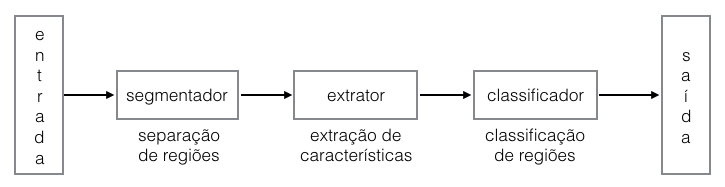
\includegraphics[width=\textwidth]{imgs/arquitetura_geral}
	\end{figure}
\end{frame}

\begin{frame}[c]
	\frametitle{Metodologia: Entrada}
	\begin{figure}[h]
    	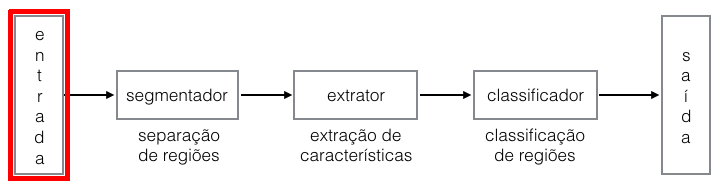
\includegraphics[width=\textwidth]{imgs/arquitetura_1}
	\end{figure}
\end{frame}

\begin{frame}[c] 
	\frametitle{Metodologia: Entrada}
	
	Imagens aéreas da floresta amazônica são a entrada para a solução.

	\vspace{0.5cm}

	Não é esperado qualquer tipo de tratamento ou filtragem prévia das imagens.
\end{frame}

\begin{frame}[c]
	\frametitle{Metodologia: Segmentador}
	\begin{figure}[h]
    	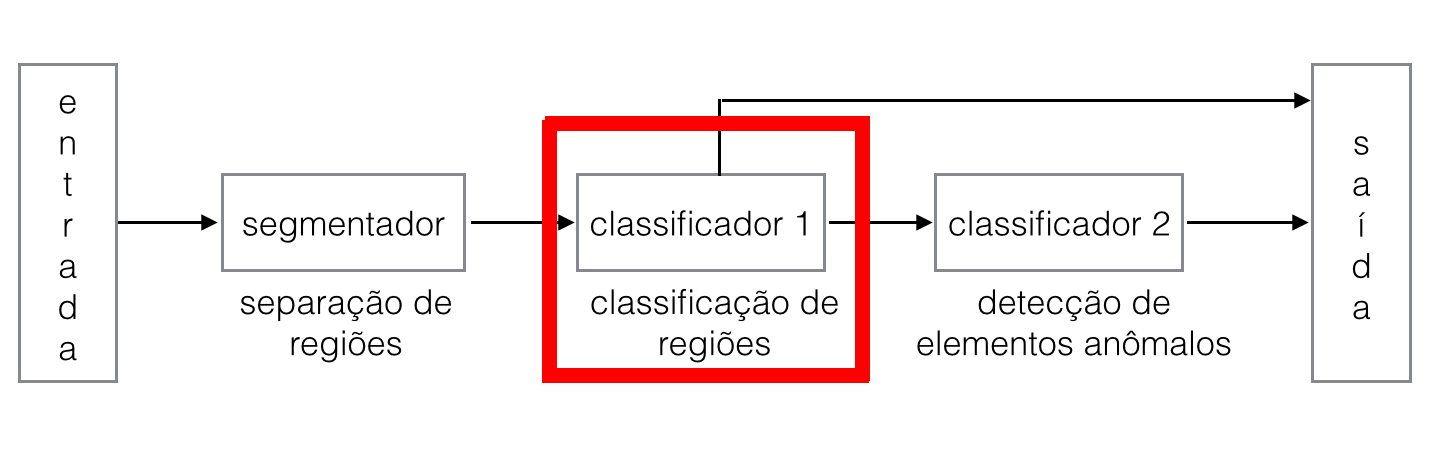
\includegraphics[width=\textwidth]{imgs/arquitetura_2}
	\end{figure}
\end{frame}

\begin{frame}[c]
	\frametitle{Metodologia: Segmentador}

	Nesta etapa, diversos métodos de segmentação de imagens são testados e seus resultados comparados.

	\vspace{0.5cm}

	Neste trabalho foram utilizados os seguintes métodos:
	\begin{itemize}
		\item FSEG;
		\item gPb-owt-ucm;
		\item JSEG;
		\item Mean-shift;
		\item MSEG;
		\item SRM;
	\end{itemize}

\end{frame}

\begin{frame}[c]
	\frametitle{Metodologia: Extrator}
	\begin{figure}[h]
    	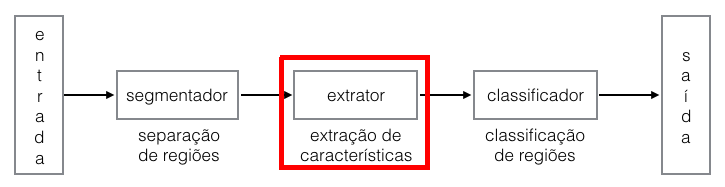
\includegraphics[width=\textwidth]{imgs/arquitetura_3}
	\end{figure}
\end{frame}

\begin{frame}[c]

	\frametitle{Metodologia: Extrator}

	Nesta etapa são extraídas informações sobre cor, intensidade, textura e morfologia das imagens. A escolha das características foi baseada nas utilizadas em trabalhos relacionados:

	\begin{itemize}
		\item Canais de cores (RBG, HSV)
		\item Histogramas de intensidade
		\item \textit{Local Binary Patterns}
		\item Transformada de Hough
	\end{itemize}
\end{frame}

\begin{frame}[c]

	\frametitle{Metodologia: Extrator}

	O algoritmo de seleção de características CFS é utilizado, e os resultados comparados ao conjunto total de características.

	\vspace{0.5cm}

	\begin{equation*}
		\displaystyle p(C=c|V_i=v_i) \neq p(C=c)
	\end{equation*}
\end{frame}

\begin{frame}[c]
	\frametitle{Metodologia: Classificador}
	\begin{figure}[h]
    	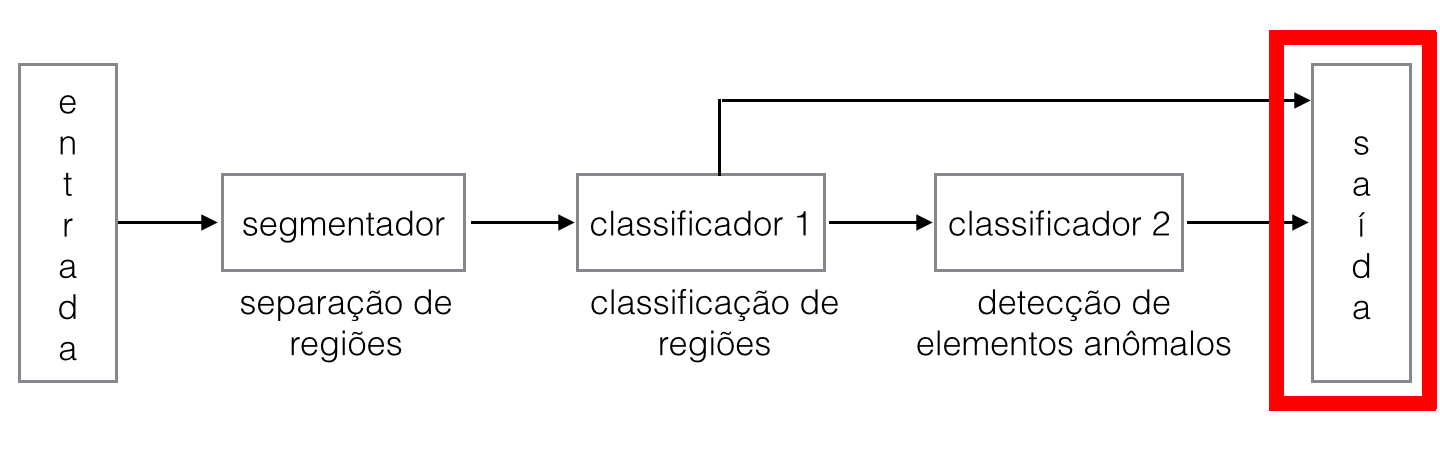
\includegraphics[width=\textwidth]{imgs/arquitetura_4}
	\end{figure}
\end{frame}

\begin{frame}[c]
	\frametitle{Metodologia: Classificador}
	
	Quatro abordagens de classificação:
	\begin{itemize}
		\item Multiclasse;
		\item Biclasse;
		\item Unária;
		\item Conjunto de unários.
	\end{itemize}
\end{frame}

\begin{frame}[c]
	\frametitle{Metodologia: Saída}
	\begin{figure}[h]
    	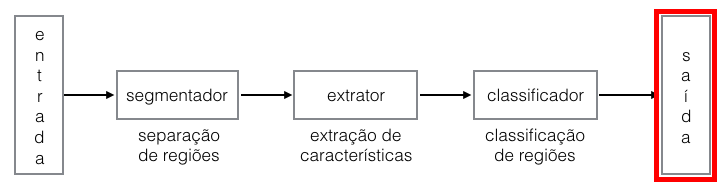
\includegraphics[width=\textwidth]{imgs/arquitetura_5}
	\end{figure}
\end{frame}

\begin{frame}[c]
	\frametitle{Metodologia: Saída}

	O resultado final do processo é uma indicação de quais segmentos da imagem são considerados elementos antrópicos.

	\vspace{0.5cm}	

	A partir do resultado final, pode ser indicado o melhor conjunto de segmentador e classificador para detecção de elementos antrópicos em imagens aéreas da floresta amazônica.
\end{frame}

%%%%%%%%%%%%%%%

\section{Experimentos}

\begin{frame}[c]
	\frametitle{Base de dados}

	\begin{itemize}
		\item 3.044 imagens em cores;
		\item Formato: JPEG;
		\item Nenhum filtro ou tratamento adicional;
		\item Dimensões: 640 x 480 pixels;
		\item 1,02 GB de dados.
	\end{itemize}

	\begin{figure}[h]
		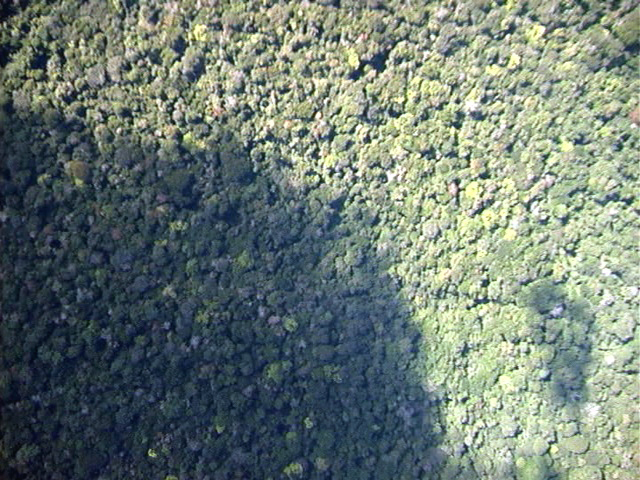
\includegraphics[width=.3\textwidth]{imgs/amostra1}
		\hspace{0.1cm}
		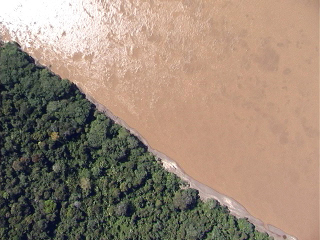
\includegraphics[width=.3\textwidth]{imgs/amostra2}
		\hspace{0.1cm}
		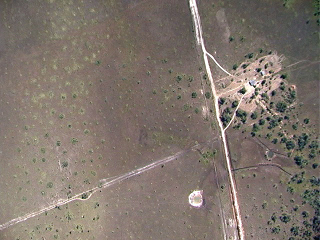
\includegraphics[width=.3\textwidth]{imgs/amostra3}
	\end{figure}

\end{frame}

\begin{frame}[c]
	\frametitle{Segmentação}

	Uma ferramenta\footnote{amazonsegmentation.ddns.net} foi construída para coletar a segmentação manual (ground-truth):

	%\vspace{0.5cm}

	\begin{minipage}{0.49\linewidth}
		\begin{itemize}
			\item 31 voluntários;
			\item 5 segmentações p/ imagem;
			\item Segmentações individuais foram fundidas;
			\item 203 imagens validadas como ground-truth.
		\end{itemize}
	\end{minipage}
	\begin{minipage}[r]{0.49\linewidth}
		\begin{figure}[h]
			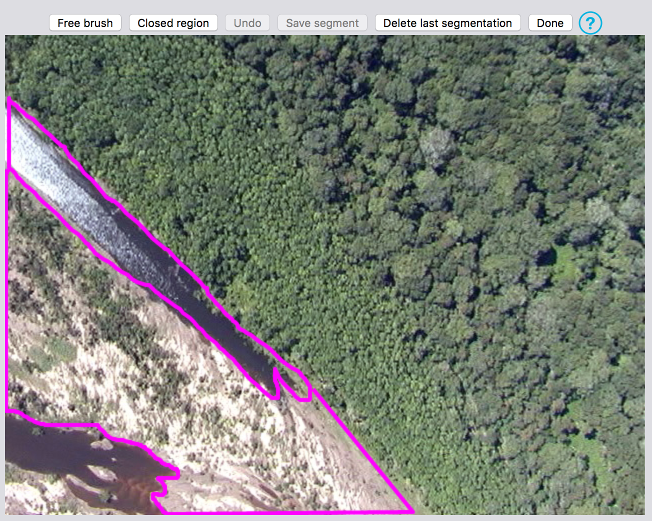
\includegraphics[width=\textwidth]{imgs/manualseg}
		\end{figure}
	\end{minipage}
\end{frame}

\begin{frame}[c]
	\frametitle{Metodologia: Segmentador}

	\begin{figure}[h]
		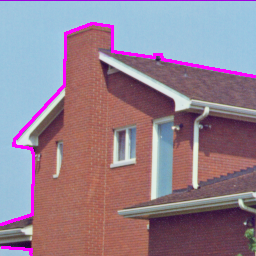
\includegraphics[width=.25\textwidth]{imgs/granularidade_1}
		\hspace{0.1cm}
		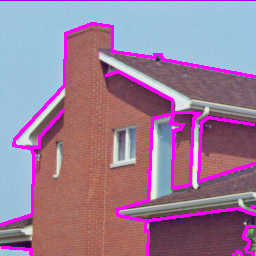
\includegraphics[width=.25\textwidth]{imgs/granularidade_2}
		\hspace{0.1cm}
		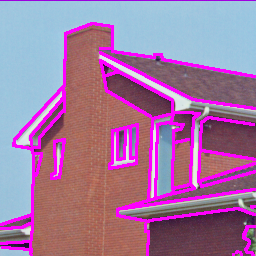
\includegraphics[width=.25\textwidth]{imgs/granularidade_3}
	\end{figure}

	Se $S_1$ e $S_2$ são duas segmentações de uma mesma imagem.	O erro de consistência entre $S_1$ e $S_2$ para uma região que contém o pixel $p_i$ é dado por:
	
	\begin{equation*}
		\displaystyle E(S_1,S_2,p_i) = \frac{|R(S_1,p_i) \setminus R(S_2,p_i)|}{|R(S_1,p_i)|}
	\end{equation*}
\end{frame}

\begin{frame}[c]
	\frametitle{Metodologia: Segmentador}

	As taxas de erro de consistência local (LCE) e global (GCE) (Martin et al., 2001) avaliam a qualidade da segmentação.

	\vspace{0.5cm}

	\begin{equation*}
		\displaystyle GCE(S_1,S_2) = \frac{1}{n} min \biggl\{ \sum_{i} E(S_1,S_2,p_i), \sum_{i} E(S_2,S_1,p_i) \biggr\}
	\end{equation*}

	\begin{equation*}
		\displaystyle LCE(S_1,S_2) = \frac{1}{n} \sum_{i} min \biggl\{ E(S_1,S_2,p_i), E(S_2,S_1,p_i) \biggr\}
	\end{equation*}
\end{frame}

\begin{frame}[c]
	\frametitle{Segmentação}
	Validação estatística da segmentação manual
	\begin{figure}[h]
		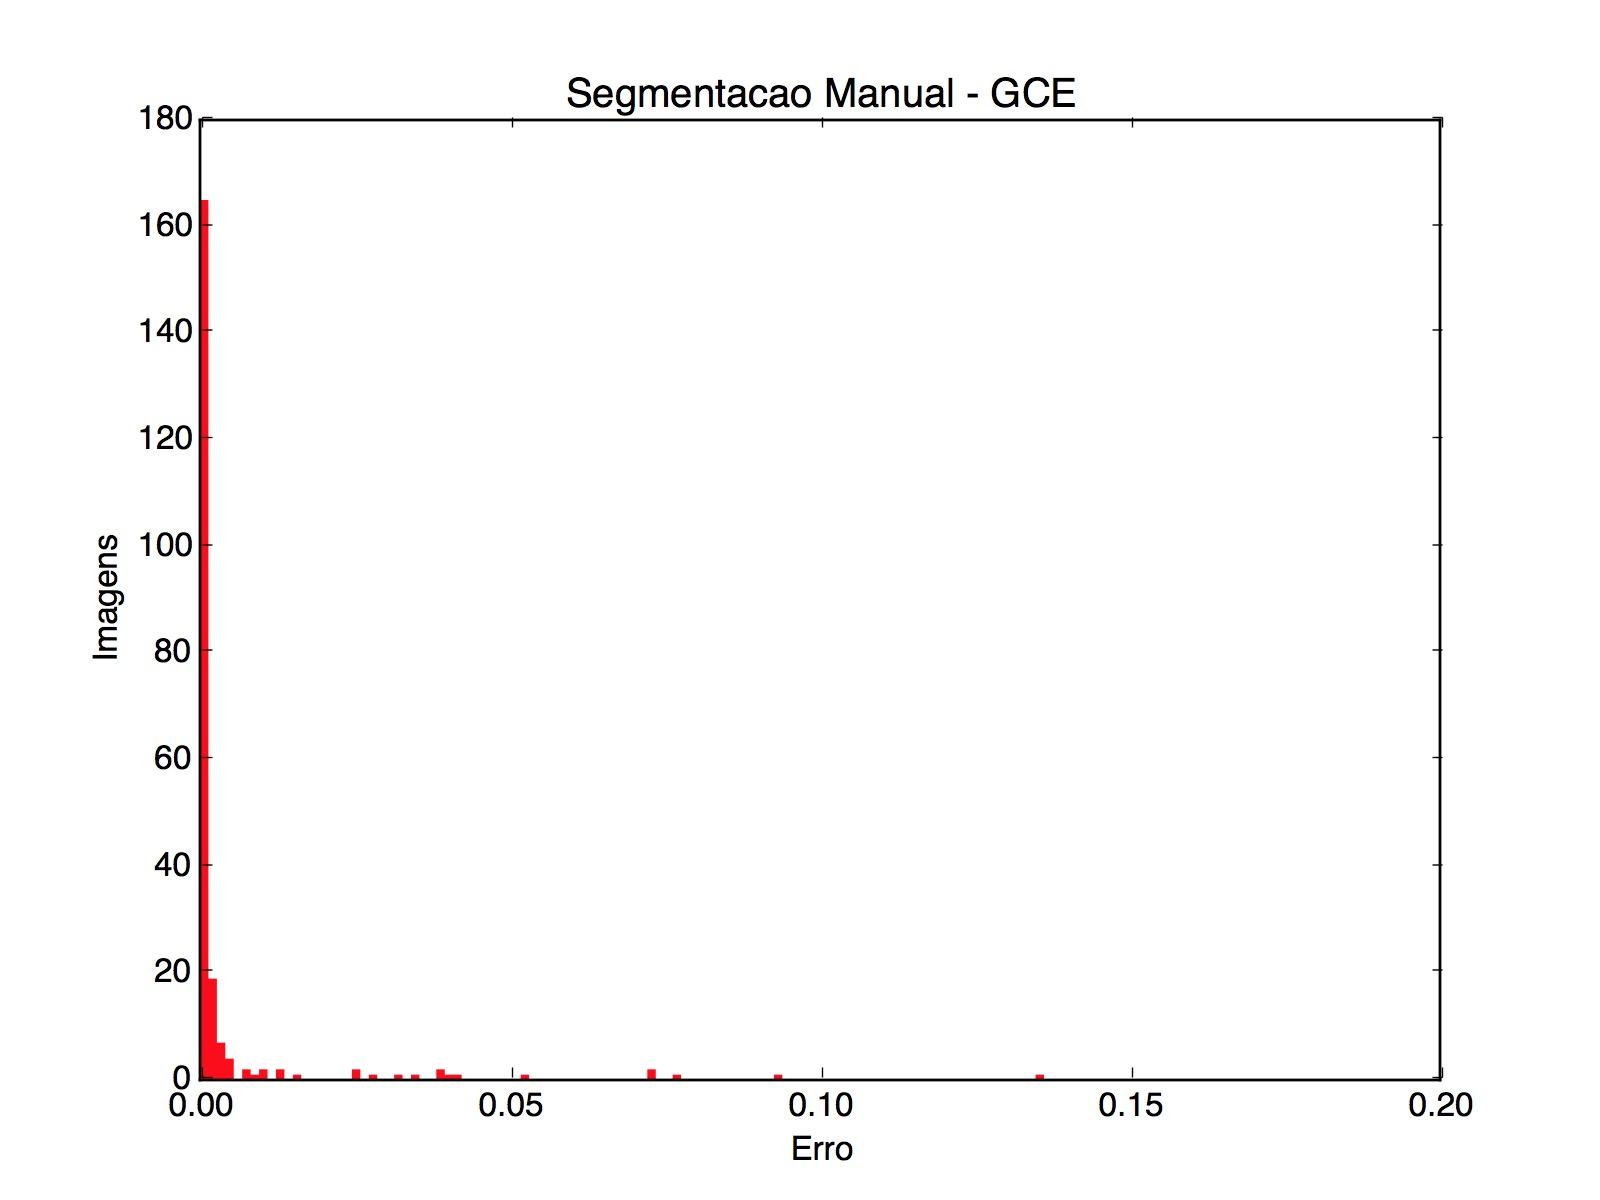
\includegraphics[scale=0.18]{imgs/manual_gce}
	\end{figure}
\end{frame}

\begin{frame}[c]
	\frametitle{Segmentação}
	Validação estatística da segmentação manual
	\begin{figure}[h]
		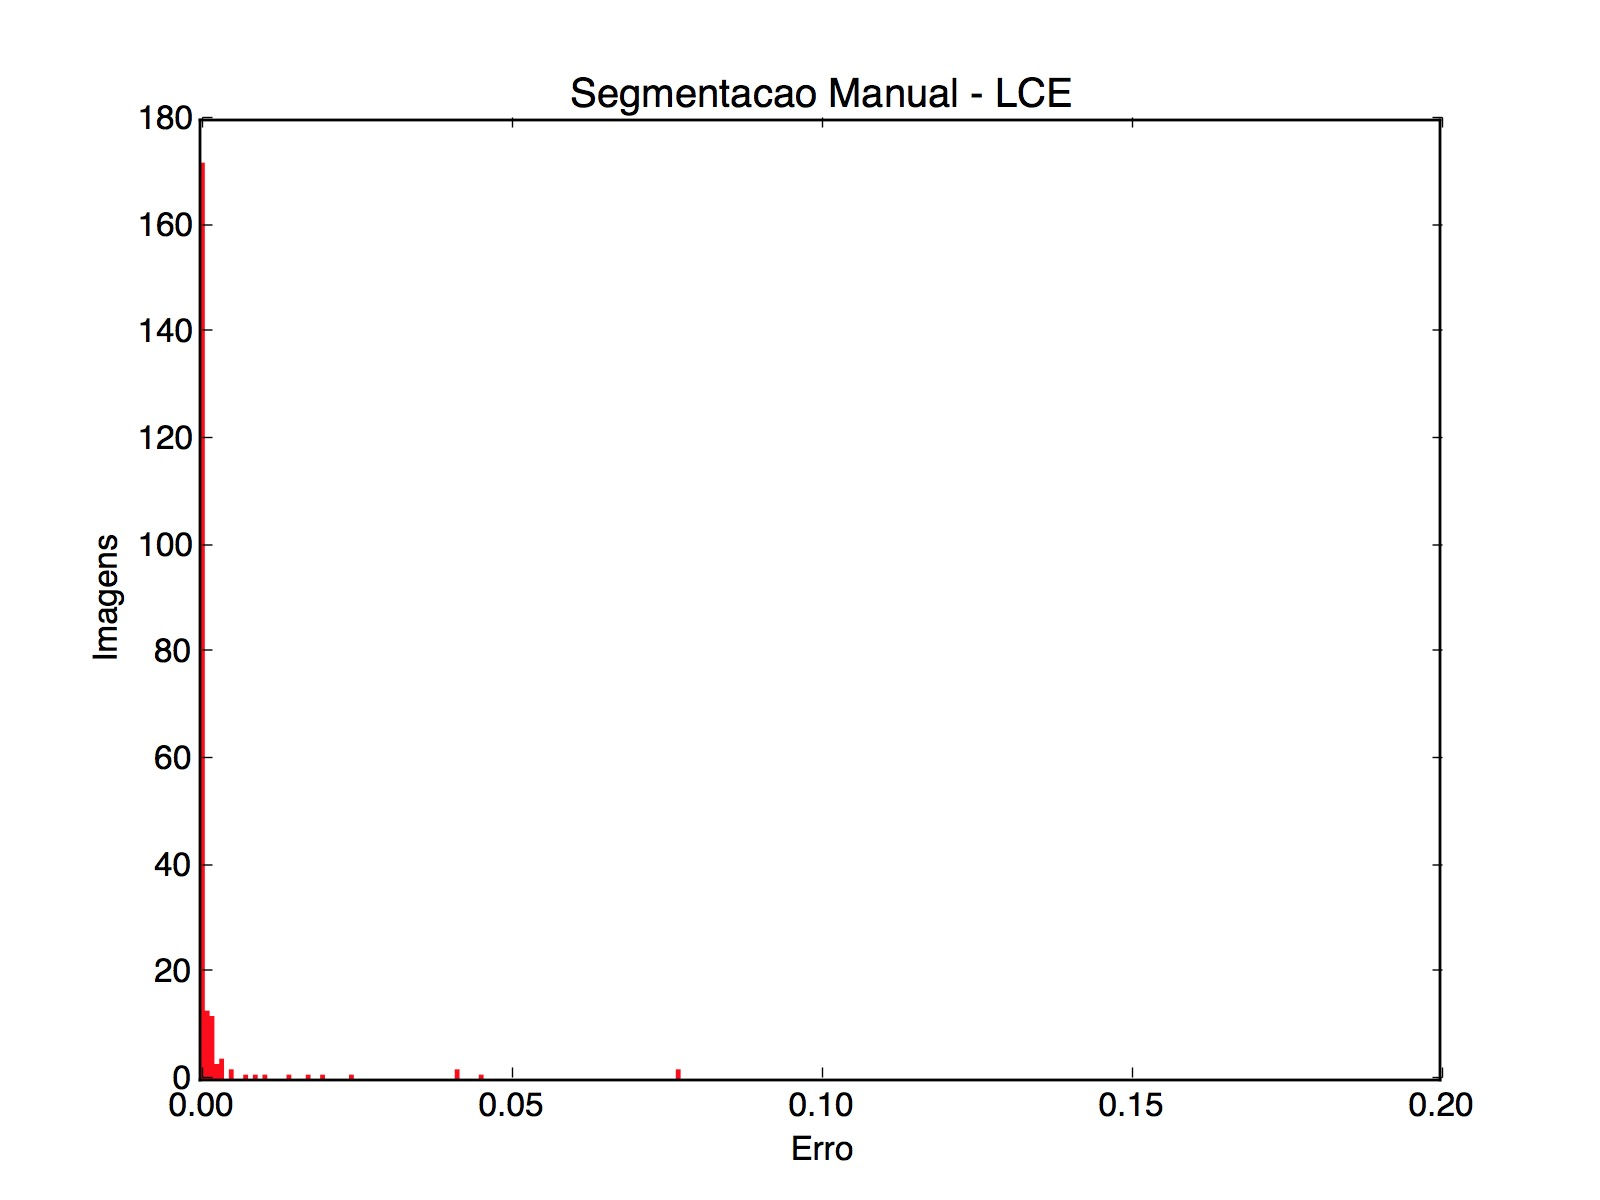
\includegraphics[scale=0.18]{imgs/manual_lce}
	\end{figure}
\end{frame}


\begin{frame}[c]
	\frametitle{Segmentação}

	\begin{figure}[c]
  		\centering
		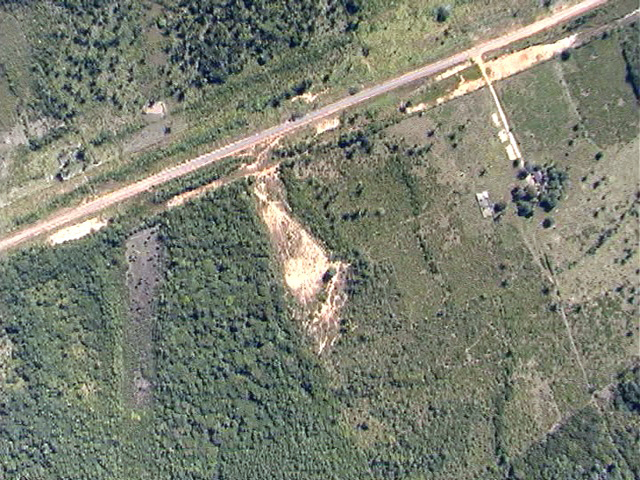
\includegraphics[width=0.8\textwidth]{imgs/seg_original}
	\end{figure}

\end{frame}

\begin{frame}[c]
	\frametitle{Segmentação}

	\begin{figure}[c]
		\centering
		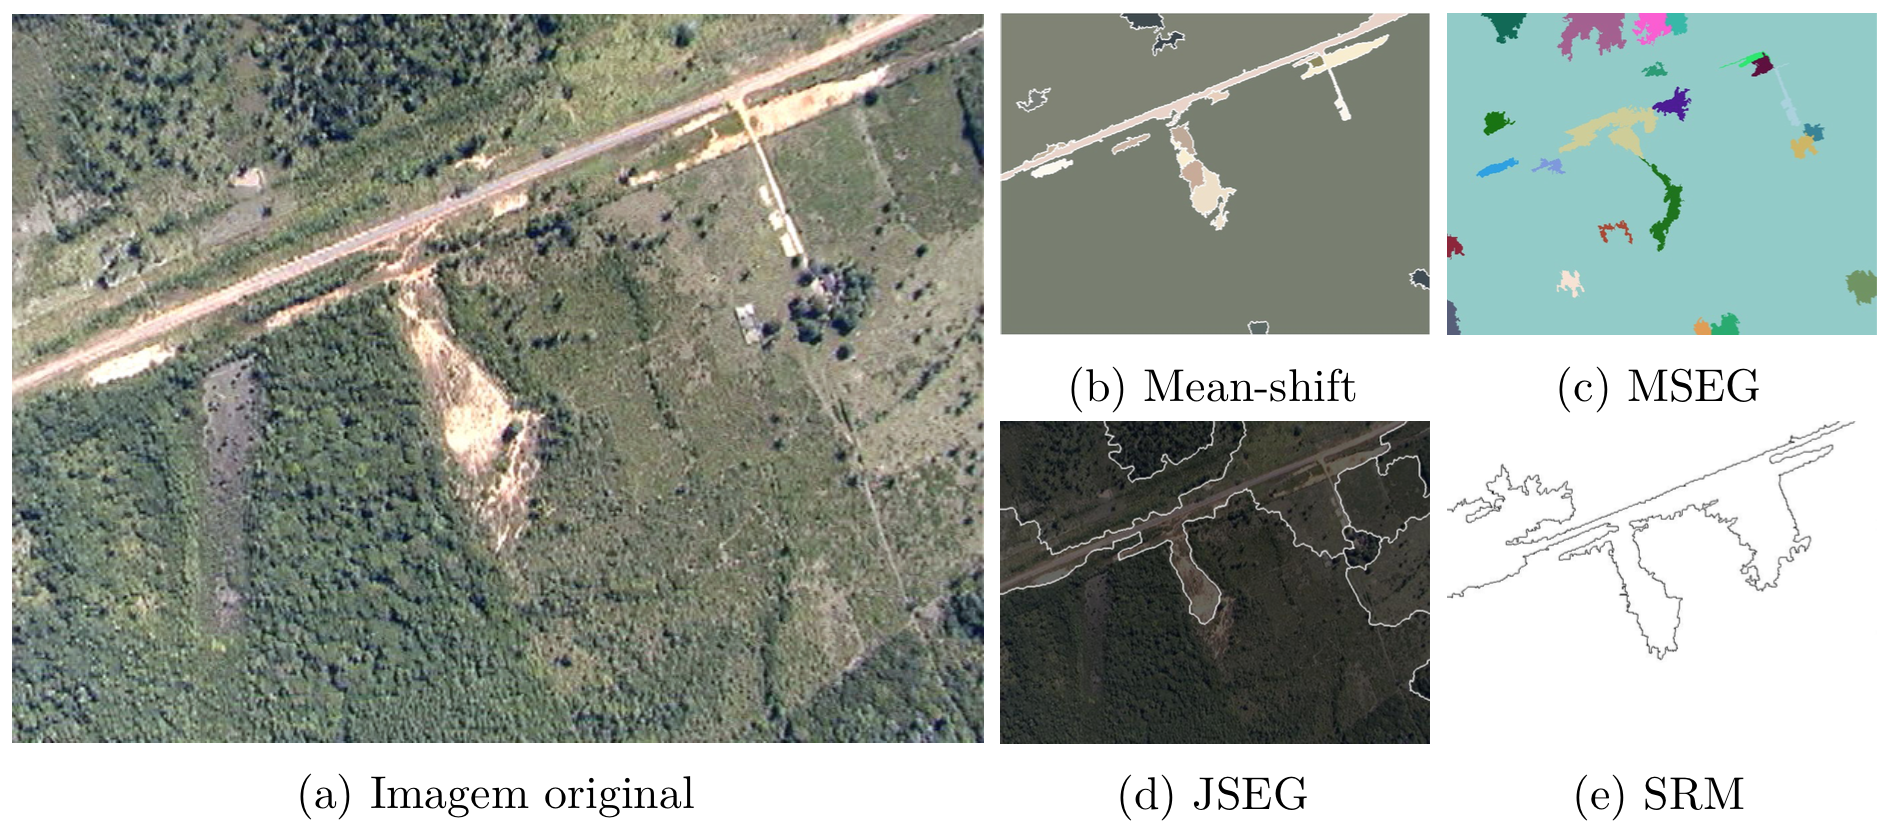
\includegraphics[width=\textwidth]{imgs/gambi_apresentacao}
	\end{figure}

\end{frame}

\begin{frame}[c]
	\frametitle{Segmentação}

	Resultados do cálculo dos erros de consistência local e global (Martin et al., 2001) para as 203 imagens utilizadas no benchmark:

	\small{
	\begin{table}[h]
		\begin{tabulary}{\linewidth}{|L|R|R|R|}
		\hline
			\textbf{Algoritmo} & \textbf{GCE médio} & \textbf{LCE médio} & \textbf{Tempo/img(s)} \\ \hline
%			Manual      & 0.01822          & 0.00537         & - \\ \hline
			FSEG        & 0.03063          & 0.00273         & 13,91 \\ \hline
			gPb-owt-ucm & 0.00655          & 0.00297         & 237,32 \\ \hline
			JSEG        & 0.02990          & 0.00486         & 14,82 \\ \hline
			Mean-shift  & 0.02237          & 0.00271         & 6,39 \\ \hline
			MSEG        & 0.01005          & 0.00072         & \cellcolor{gray!25} 0,33 \\ \hline
			SRM         & \cellcolor{gray!25} 0.00622 & \cellcolor{gray!25} 0.00066 & 4,66 \\ \hline
		\end{tabulary}
	\end{table}
	}
\end{frame}

%\begin{frame}
%	\frametitle{Segmentação}
%
%	Um experimento para realizar segmentação e a primeira classificação em uma única etapa foi realizado, um artigo sobre o experimento foi publicado  na conferência VISAPP 2015. 
%
%	\small{
%	\begin{table}
%	\centering
%	\begin{tabulary}{\linewidth}{|L|R|R|}
%		\hline
%		\textbf{Algoritmo} & \textbf{Acurácia} & \textbf{Tempo/imagem} \\ \hline
%		Random forest  & 96,0\% & 12,72 s \\ \hline
%		KNN            & 92,6\% & 22,89 s \\ \hline
%		Naive Bayes    & 92,8\% & 8,36 s \\ \hline
%		Decision tree  & 82,2\% & 14,49 s \\ \hline
%	\end{tabulary}
%	\end{table}
%	}
%
%\end{frame}

\begin{frame}[c]
	\frametitle{Classificação}

	Todas as imagens da base foram segmentadas com o método SRM\\
	\vspace{0.5cm}
	3.044 imagens $\Rightarrow$ 10.057 segmentos\\
	\vspace{0.5cm}
	Todos os segmentos foram manualmente rotulados em: Floresta, água, vegetação rasteira, terra e elemento antrópico.
	\vspace{0.2cm}

	\centering
	Vetor de características
	\small{
		\begin{table}[h]
		\centering
		\begin{tabulary}{\linewidth}{|L|L|R|}
		\hline
		\textbf{Atributo} & \textbf{Tipo} & \textbf{Dimensão} \\ \hline
		Vermelho médio            & Real    &  1 \\ \hline
		Verde médio               & Real    &  1 \\ \hline
		Azul médio                & Real    &  1 \\ \hline
		Intensidade média         & Real    &  1 \\ \hline
		Intensidade - histograma  & Inteiro & 16 \\ \hline
		LBP - histograma          & Inteiro & 26 \\ \hline
		Hough - número de retas   & Inteiro &  1 \\ \hline
		Hough - maior reta        & Inteiro &  1 \\ \hline
		\end{tabulary}
		\end{table}
	}

	\centering
	Base disponível em \textbf{github.com/luizcavalcanti/geoma-database}.

\end{frame}

\begin{frame}[c]
	\frametitle{Classificação - Avaliação}

	Para comparação dos resultados de classificação, os valores de precisão, revocação e medida F1 para todas as classes e para a classe de interesse (elementos antrópicos) foram avaliados:

	\begin{equation*}
		\displaystyle Pr = \frac{TP}{TP+FP}
	\end{equation*}

	\begin{equation*}
		\displaystyle Rv = \frac{TP}{TP+FN}
	\end{equation*}

	\begin{equation*}
		\displaystyle F_1 = 2 \cdot \frac{Pr \cdot Rv}{Pr + Rv}
	\end{equation*}

	\vspace{0.5cm}	

	Todos os experimentos foram realizados com e sem seleção de características através do método CFS.
\end{frame}

\begin{frame}[c]
	\frametitle{Classificação - Multiclasse}

	Base rotulada e dividida entre 5 classes:
	\vspace{0.3cm}
	\begin{itemize}
		\begin{minipage}{0.4\linewidth}
			\item Floresta;
			\item Água;
			\item Vegetação rasteira;
		\end{minipage}
		\begin{minipage}{0.4\linewidth}
			\item Terra;
			\item Elementos antrópicos.
		\end{minipage}
	\end{itemize}

	\vspace{0.5cm}

	Algoritmos:
	\begin{itemize}
		\item Random Forest;
		\item Árvores de decisão;
		\item KNN;
		\item SVM;
		\item Naive Bayes.
	\end{itemize}
\end{frame}

\begin{frame}[c]
	\frametitle{Classificação - Multiclasse}

	\centering
	Distribuição de classes

	\small{
	\begin{table}[h]
	\centering
	\begin{tabulary}{\linewidth}{|L|R|R|}
		\hline
		\textbf{Classe} & \textbf{Amostras} & \textbf{Percentual} \\ \hline
		Floresta             & 8.684 & 86,3\% \\ \hline
		Vegetação rasteira   & 939   &  9,3\% \\ \hline
		Água                 & 287   &  2,8\% \\ \hline
		Clareira             & 136   &  1,3\% \\ \hline
		Elementos antrópicos & 31    &  0,3\% \\ \hline
	\end{tabulary}
	\end{table}
	}

	\centering
	Vetor de características após seleção via CFS

	\small{
	\begin{table}[h]
	\centering
	\begin{tabulary}{\linewidth}{|L|L|R|}
	\hline
	\textbf{Atributo} & \textbf{Tipo} & \textbf{Dimensão} \\ \hline
	Intensidade - histograma (5/15) & Inteiro & 5 \\ \hline
	LBP - histograma (1/26)         & Inteiro & 1 \\ \hline
	Hough - maior reta              & Inteiro & 1 \\ \hline
	\end{tabulary}
	\end{table}
	}
\end{frame}

\begin{frame}[c]
	\frametitle{Classificação - Multiclasse}

	\centering
	Resultados para \textbf{todas as classes}

	\small{
	\begin{table}[h]
		\centering
		\begin{tabulary}{\linewidth}{|L|R|R|R|}
			\hline
			\textbf{Método} & \textbf{Precisão} & \textbf{Revocação} & \textbf{F1} \\ \hline
			Random Forest          & \cellcolor{gray!25}0.917 & \cellcolor{gray!25}0.930 & \cellcolor{gray!25}0.921 \\ \hline
			KNN                     & 0.907 & 0.920 & 0.909 \\ \hline
			SVM                     & 0.899 & 0.915 & 0.900 \\ \hline
			Random Forest (CFS)     & 0.893 & 0.910 & 0.899 \\ \hline
			Árvore de decisão             & 0.898 & 0.904 & 0.901 \\ \hline
			KNN (CFS)               & 0.880 & 0.898 & 0.887 \\ \hline
			Árvore de decisão (CFS) & 0.880 & 0.894 & 0.886 \\ \hline
			SVM (CFS)               & 0.798 & 0.866 & 0.808 \\ \hline
			Naive Bayes (CFS)       & 0.845 & 0.816 & 0.824 \\ \hline
			Naive Bayes             & 0.857 & 0.563 & 0.101 \\ \hline
		\end{tabulary}
	\end{table}
	}
\end{frame}

\begin{frame}[c]
	\frametitle{Classificação - Multiclasse}

	\centering
	Resultados para a classe de \textbf{elementos antrópicos}

	\small{
		\begin{table}[h]
		\centering
		\begin{tabulary}{\linewidth}{|L|R|R|R|}
		\hline
		\textbf{Método} & \textbf{Precisão} & \textbf{Revocação} & \textbf{F1} \\ \hline
		KNN                     & 0.889 & 0.727 & \cellcolor{gray!25}0.800 \\ \hline
		Random Forest           & \cellcolor{gray!25}0.917 & 0.500 & 0.647 \\ \hline
		SVM (CFS)               & 0.813 & 0.591 & 0.684 \\ \hline
		Árvore de decisão       & 0.700 & 0.636 & 0.667 \\ \hline
		Random Forest (CFS)     & 0.846 & 0.500 & 0.629 \\ \hline
		KNN (CFS)               & 0.722 & 0.591 & 0.650 \\ \hline
		Árvore de decisão (CFS) & 0.588 & 0.455 & 0.513 \\ \hline
		Naive Bayes             & 0.054 & \cellcolor{gray!25}0.955 & 0.101 \\ \hline
		Naive Bayes (CFS)       & 0.030 & 0.909 & 0.058 \\ \hline
		SVM                     & 0.030 & 0.591 & 0.057 \\ \hline
		\end{tabulary}
		\end{table}
	}
\end{frame}


\begin{frame}[c]
	\frametitle{Classificação - Biclasse}

	Base rotulada e dividida entre 2 classes:
	\vspace{0.3cm}
	\begin{itemize}
		\item Elementos naturais;
		\item Elementos antrópicos.
	\end{itemize}

	\vspace{0.5cm}

	Algoritmos:
	\begin{itemize}
		\item Random Forest;
		\item Árvores de decisão;
		\item KNN;
		\item SVM;
		\item Naive Bayes.
	\end{itemize}

\end{frame}

\begin{frame}[c]
	\frametitle{Classificação - Biclasse}

	\centering
	Distribuição de classes

	\small{
		\begin{table}[h]
		\centering
		\begin{tabulary}{\linewidth}{|L|R|R|}
		\hline
		\textbf{Classe} & \textbf{Amostras} & \textbf{Percentual} \\ \hline
		Elementos naturais   & 10.026 & 99,7 \% \\ \hline
		Elementos antrópicos &     31 &  0,3 \% \\ \hline
		\end{tabulary}
	\end{table}
	}

	\centering
	Vetor de características após seleção via CFS

	\small{
		\begin{table}[h]
		\centering
		\begin{tabulary}{\linewidth}{|L|L|R|}
		\hline
		\textbf{Atributo} & \textbf{Tipo} & \textbf{Dimensão} \\ \hline
		Intensidade - histograma (5/15) & Inteiro & 5 \\ \hline
		LBP - histograma (1/26)         & Inteiro & 1 \\ \hline
		Hough - maior reta              & Inteiro & 1 \\ \hline
		\end{tabulary}
		\end{table}
	}

\end{frame}

\begin{frame}[c]
	\frametitle{Classificação - Biclasse}

	\centering
	Resultados para \textbf{todas as classes}

	\small{
		\begin{table}[h]
		\centering
		\begin{tabulary}{\linewidth}{|L|R|R|R|R|}
			\hline
			\textbf{Método} & \textbf{Precisão} & \textbf{Revocação} & \textbf{F1} \\ \hline
			KNN (CFS)               & \cellcolor{gray!25}0.999 & \cellcolor{gray!25}0.999 & \cellcolor{gray!25}0.999 \\ \hline
			Random Forest           & 0.999 & 0.999 & 0.999 \\ \hline
			KNN                     & 0.999 & 0.999 & 0.999 \\ \hline
			Random Forest (CFS)     & 0.998 & 0.998 & 0.998 \\ \hline
			Árvore de decisão       & 0.999 & 0.999 & 0.999 \\ \hline
			Árvore de decisão (CFS) & 0.999 & 0.999 & 0.999 \\ \hline
			SVM (CFS)               & 0.999 & 0.999 & 0.999 \\ \hline
			SVM                     & 0.995 & 0.997 & 0.996 \\ \hline
			Naive Bayes (CFS)       & 0.997 & 0.973 & 0.984 \\ \hline
			Naive Bayes             & 0.997 & 0.939 & 0.966 \\ \hline
		\end{tabulary}
	\end{table}
	}
\end{frame}

\begin{frame}[c]
	\frametitle{Classificação - Biclasse}

	\centering
	Resultados para a classe de \textbf{elementos antrópicos}

	\small{
		\begin{table}[h]
		\centering
		\begin{tabulary}{\linewidth}{|L|R|R|R|R|}
		\hline
		\textbf{Método} & \textbf{Precisão} & \textbf{Revocação} & \textbf{F1} \\ \hline
		KNN (CFS)               & \cellcolor{gray!25}1.000 & 0.615 & \cellcolor{gray!25}0.762 \\ \hline
		Random Forest           & 0.941 & 0.615 & 0.744 \\ \hline
		Árvore de decisão (CFS) & 0.941 & 0.615 & 0.744 \\ \hline
		SVM (CFS)               & 0.889 & 0.615 & 0.727 \\ \hline
		Árvore de decisão       & 0.842 & 0.615 & 0.711 \\ \hline
		KNN                     & 0.733 & 0.654 & 0.708 \\ \hline
		Random Forest (CFS)     & 0.727 & 0.615 & 0.667 \\ \hline
		Naive Bayes (CFS)       & 0.075 & 0.846 & 0.137 \\ \hline
		Naive Bayes             & 0.039 & \cellcolor{gray!25}0.962 & 0.076 \\ \hline
		SVM                     & 0.030 & 0.591 & 0.057 \\ \hline
		\end{tabulary}
		\end{table}
	}
\end{frame}

\begin{frame}[c]
	\frametitle{Classificação - Unária}

	Base dividida em 2 classes, mas parcialmente rotulada para apenas uma classe:
	\vspace{0.3cm}
	\begin{itemize}
		\item Elementos naturais (target);
		\item Elementos antrópicos (outlier).
	\end{itemize}

	\vspace{0.5cm}

	Algoritmos:
	\begin{itemize}
		\item OC-SVM;
		\item REPTree.
	\end{itemize}

\end{frame}

\begin{frame}[c]
	\frametitle{Classificação - Unária}
	
	\centering
	Distribuição de classes

	\small{
		\begin{table}[h]
		\centering
		\begin{tabulary}{\linewidth}{|L|R|R|}
		\hline
		\textbf{Classe} & \textbf{Amostras} & \textbf{Percentual} \\ \hline
		Elementos naturais (target)    & 10.026 & 99,7 \% \\ \hline
		Elementos antrópicos (outlier) &     31 &  0,3 \% \\ \hline
		\end{tabulary}
	\end{table}
	}

	\centering
	Vetor de características após seleção via CFS

	\small{
		\begin{table}[h]
		\centering
		\begin{tabulary}{\linewidth}{|L|L|R|}
		\hline
		\textbf{Atributo} & \textbf{Tipo} & \textbf{Dimensão} \\ \hline
		Intensidade - histograma (1/15) & Inteiro & 1 \\ \hline
		Hough - maior reta              & Inteiro & 1 \\ \hline
		\end{tabulary}
		\end{table}
	}
	
\end{frame}

\begin{frame}[c]
	\frametitle{Classificação - Unária}

	\centering
	Resultados para \textbf{todas as classes}

	\small{
		\begin{table}[h]
		\centering
		\begin{tabulary}{\linewidth}{|L|R|R|R|R|}
		\hline
		\textbf{Método} & \textbf{Precisão} & \textbf{Revocação} & \textbf{F1} \\ \hline
		OC-SVM (CFS)  & \cellcolor{gray!25}0.999 & \cellcolor{gray!25}0.999 & \cellcolor{gray!25}0.999 \\ \hline
		OC-SVM        & 0.995 & 0.997 & 0.996 \\ \hline
		REPTree       & 0.996 & 0.465 & 0.632 \\ \hline
		REPTree (CFS) & 0.997 & 0.384 & 0.552 \\ \hline
		\end{tabulary}
		\end{table}
	}

	\centering
	Resultados para a classe de \textbf{elementos antrópicos}

	\small{
		\begin{table}[h]
		\centering
		\begin{tabulary}{\linewidth}{|L|R|R|R|}
		\hline
		\textbf{Método} & \textbf{Precisão} & \textbf{Revocação} & \textbf{F1} \\ \hline
		OC-SVM (CFS)  & \cellcolor{gray!25}0.842 & 0.615 & \cellcolor{gray!25}0.711 \\ \hline
		REPTree (CFS) & 0.004 & \cellcolor{gray!25}0.962 & 0.008 \\ \hline
		REPTree       & 0.003 & 0.692 & 0.007 \\ \hline
		OC-SVM        & 0.000 & 0.000 & 0.000 \\ \hline
		\end{tabulary}
		\end{table}
	}
\end{frame}

\begin{frame}[c]
	\frametitle{Classificação - Conjunto de unários}

	Diversas bases criadas, uma para cada classificador a ser treinado, levando em consideração a classe de interesse no contexto e a classe anômala.

	\vspace{0.5cm}

	Os métodos devem ser combinados e o resultado final de classificação deve se dar por votação com pesos.

	\vspace{0.5cm}

	Algoritmos:
	\begin{itemize}
		\item OC-SVM;
		\item REPTree.
	\end{itemize}
\end{frame}

\begin{frame}[c]
	\frametitle{Classificação - Conjunto de unários}

	\centering
	Vetor de características após seleção via CFS

	\small{
		\begin{table}[h]
		\centering
		\begin{tabulary}{\linewidth}{|L|L|R|}
		\hline
		\textbf{Classe majoritária} & \textbf{Atributo} & \textbf{Dimensão} \\ \hline
		\multirow{3}{*}{Floresta} & Intensidade - histograma (5/15) & 7 \\ \cline{2-3}
        		                  & LBP - histograma (1/26)         & 1 \\ \cline{2-3}
                			          & Hough - maior reta              & 1 \\ \hline \hline
		\multirow{3}{*}{Água}     & Intensidade - histograma (7/15) & 7 \\ \cline{2-3}
        		                  & LBP - histograma (2/26)         & 2 \\ \cline{2-3}
	                		          & Hough - número de retas         & 1 \\ \hline \hline
		\multirow{3}{*}{Vegetação}& Intensidade - histograma (6/15) & 7 \\ \cline{2-3}
        		                  & LBP - histograma (1/26)         & 1 \\ \cline{2-3}
                			          & Hough - número de retas         & 1 \\ \hline \hline
		\multirow{4}{*}{Terra}    & Intensidade - histograma (7/15) & 7 \\ \cline{2-3}
        		                  & LBP - histograma (1/26)         & 1 \\ \cline{2-3}
                		        		  & Hough - número de retas         & 1 \\ \cline{2-3}
                    			      & Hough - maior reta              & 1 \\ \hline
		\end{tabulary}
		\end{table}
	}

\end{frame}

\begin{frame}[c]
	\frametitle{Classificação - Conjunto de unários}

	\centering
	Resultados para classificadores individuais

	\small{
		\begin{table}[h]
		\centering
		\begin{tabulary}{\linewidth}{|L|R|R|R|}
		\hline
		\textbf{Classe/Algoritmo} & \textbf{Precisão} & \textbf{Revocação} & \textbf{F1} \\ \hline
		Floresta/OCSVM         & 0.941 & 0.943 & 0.939 \\ \hline
		Floresta/OCSVM (CFS)   & 0.941 & 0.943 & 0.939 \\ \hline
		Floresta/REPTree        & 0.847 & 0.856 & 0.792 \\ \hline
		Floresta/REPTree (CFS)  & 0.821 & 0.805 & 0.812 \\ \hline
		Água/OCSVM             & 0.971 & 0.976 & 0.969 \\ \hline
		Água/OCSVM (CFS)       & 0.353 & 0.763 & 0.482 \\ \hline
		Água/REPTree            & 0.954 & 0.538 & 0.675 \\ \hline
		Água/REPTree (CFS)      & 0.952 & 0.445 & 0.590 \\ \hline
		Vegetação/OCSVM        & 0.920 & 0.930 & 0.919 \\ \hline
		Vegetação/OCSVM (CFS)  & 0.433 & 0.871 & 0.578 \\ \hline
		Vegetação/REPTree       & 0.837 & 0.539 & 0.633 \\ \hline
		Vegetação/REPTree (CFS) & 0.887 & 0.333 & 0.407 \\ \hline
		Terra/OCSVM            & 0.983 & 0.987 & 0.981 \\ \hline
		Terra/OCSVM (CFS)      & 0.954 & 0.453 & 0.614 \\ \hline
		Terra/REPTree           & 0.980 & 0.305 & 0.452 \\ \hline
		Terra/REPTree (CFS)     & 0.979 & 0.363 & 0.519 \\ \hline
		\end{tabulary}
		\end{table}
	}
\end{frame}

\begin{frame}[c]
	\frametitle{Classificação - Conjunto de unários}

	Pesos utilizados:
	\begin{itemize}
		\item Floresta = 0.5
		\item Água = 0.3
		\item Vegetação = 0.1
		\item Terra = 0.1
	\end{itemize}

	Melhores resultados dentre as combinações de classificadores, para a classe de \textbf{elementos antrópicos}:

	\small{
		\begin{table}[h]
		\centering
		\begin{tabulary}{\linewidth}{|C|C|C|C|C|C|C|}
		\hline
		\textbf{Flor.} & \textbf{Água} & \textbf{Veg.} & \textbf{Terra} & \textbf{Pr} & \textbf{Rv} & \textbf{F1} \\ \hline
		OS & OS (CFS) & RT       & OS       & \cellcolor{gray!25}0.947 & 0.692 & \cellcolor{gray!25}0.800 \\ \hline
		RT & OS       & RT       & RT       & 0.850 & 0.730 & 0.785 \\ \hline
		RT & OS       & OS       & RT (CFS) & 0.809 & 0.653 & 0.723 \\ \hline
		OS & RT (CFS) & OS       & OS       & 0.239 & 0.653 & 0.350 \\ \hline
		OS & OS       & RT       & OS       & 0.156 & \cellcolor{gray!25}0.769 & 0.259 \\ \hline
		OS & RT       & RT (CFS) & OS       & 0.153 & 0.653 & 0.248 \\ \hline
		\end{tabulary}
		\end{table}
	}

\end{frame}

\begin{frame}[c]
	\frametitle{Resultados}
	
	\centering
	Resultados gerais para a classe de \textbf{elementos antrópicos}

	\small{
		\begin{table}[h]
		\centering
		\begin{tabulary}{\linewidth}{|L|R|R|R|}
		\hline
		\textbf{Abordagem}  & \textbf{Precisão} & \textbf{Revocação} & \textbf{F1} \\ \hline
		Classificadores multi-classe (KNN)   & 0.889 & \cellcolor{gray!25}0.727 & \cellcolor{gray!25}0.800 \\ \hline
		Conjunto de classificadores unários  & 0.947 & 0.692 & \cellcolor{gray!25}0.800 \\ \hline
		Classificadores binários (KNN)       & \cellcolor{gray!25}1.000 & 0.615 & 0.762 \\ \hline
		Classificadores unários (OC-SVM)     & 0.842 & 0.615 & 0.711 \\ \hline
		\end{tabulary}
		\end{table}
	}

	\begin{figure}
		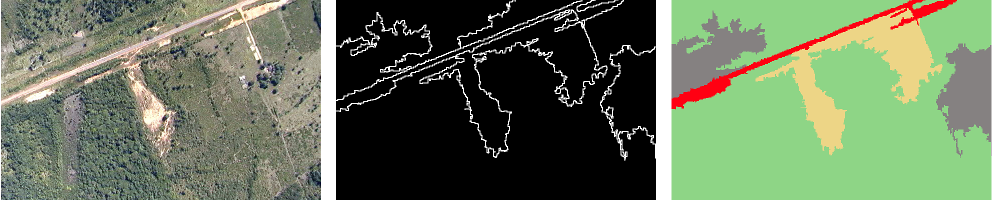
\includegraphics[width=\textwidth]{imgs/resultado_final}
	\end{figure}
\end{frame}

%%%%%%%%%%%%%%%

\section{Conclusão}

\begin{frame}[c]
	\frametitle{Conclusão}

	\begin{itemize}
		\item O algoritmo SRM obteve o menor erro de consistência dentre as técnicas de segmentação experimentadas;
		\item O conjunto de características escolhido demonstrou boa capacidade de descrição das classes do problema e a seleção de características CFS se mostrou importante em diversos casos;
		\item Embora tenha empatado com a abordagem multi-classe, o conjunto de classificadores unários obteve resultados promissores e se mostra a proposta mais robusta.
	\end{itemize}
\end{frame}

\begin{frame}[c]
	\frametitle{Contribuições}

	\begin{itemize}
		\item Criada e disponibilizada uma base de imagens aéreas da floresta amazônica e de segmentos destas mesmas imagens, devidamente rotuladas;
		\item Definido um método de segmentação adequado para o tipo de imagem do problema;
		\item Definido um conjunto de características que descrevem as classes do problema;
		\item Definido um conjunto de técnicas de aprendizado de máquina para detecção de elementos antrópicos em imagens aéreas da floresta amazônica;
%		\item A base de imagens, de segmentos e todos os algoritmos e resultados encontrados estão publicamente disponíveis e são um bom ponto de apoio a trabalhos futuros.
	\end{itemize}
\end{frame}

\begin{frame}[c]
	\frametitle{Trabalhos futuros}

	\begin{itemize}
		\item Ampliar o conjunto de imagens, a fim de reduzir o desequilíbrio das classes;
		\item Explorar outras técnicas de votação/decisão em conjuntos de classificadores;
		\item Explorar mais algoritmos para classificação unária.
	\end{itemize}
\end{frame}

\begin{frame}

	\vspace{0.4\textheight}

	\centering
	\huge Obrigado
	
	\vspace{100cm}
	
	\cite{martin:2001}
	\cite{arbelaez:2011}
	\cite{yuan2:2013}
	\cite{hall:1998}
	\cite{alpaydin:2010}
	\cite{mitchell:1997}
	\cite{gonzalez:2002}
	\cite{jain:1989}
	\cite{nixon:2008}
\end{frame}

\begin{frame}{Referências}
	\tiny{\bibliographystyle{abbrv}}
%	\tiny{\bibliographystyle{apacite}}
	\bibliographystyle{humannat}
	\bibliography{dissertacao}
\end{frame}

\end{document}